\section{Proposed conditional generative model}

We introduce a generative model framework with transformer-based auto-encoder and conditional latent diffusion model for the problem at hand. We further need to tokenize the parameter data that we have for the transformer model. Each of these components are explained in further detail in the below subsections.   

\subsection{Composite tokenizer}

For compatibility with transformer-based architectures, optical design parameters must be converted into sequence of tokens. Lens assembly can be characterized by a sequence of surfaces but each surface has a set of parameters as described in sub-section\ref{subsec:param_meth}. So each parameter is mapped to an individual token using the following process:
\begin{enumerate}
  \item \textbf{Initial embedding}
  \begin{enumerate}
    \item Numerical parameters are embedded using learnable affine projections
    \item Categorical parameters are embedded using lookup table 
  \end{enumerate}
  \item \textbf{Encoding parameter type} To enable the model to track parameter type of each token, a learnable parameter-type embedding (unique for each parameter type, same across surfaces) is added to each token based on associated parameter category.
  \item \textbf{Encoding surface position} 
  Surface ordering along the optical axis is also encoded using a relative fourier-based embedding. For the $i^{th}$ surface in a sytem with $N$ surfaces, a normalized position $\frac{i}{N-1}$ is computed and mapped to a set of sinusoidal fourier features, followed by a learned linear projection. The resulting embedding is added to the associated parameter tokens based on the surface number they belong to. 
  \item Aperture stop surface index is not included in the token sequence and instead  predicted at the decoder output using a dedicated regression head
\end{enumerate}

\subsection{Transformer based auto-encoder}
The overall encoder-decoder architecture follows a modified version of the standard transformer formulation introduced in \cite{vaswani2023attentionneed}, as shown in the figure \ref{fig:vasvani_trans}. The encoder operates on the tokens generated by the composite tokenizer described in the previous section, capturing both intra-surface parameter interactions and inter-surface relationships along optical axis. Rather than passing encoder outputs to the decoder, we aggregate them into a compact fixed dimensional latent representation using learned attention pooling. 

The decoder is implemented as an autoregressive transformer that takes in latent representation through cross-attention layers and reconstructs individual parameters in a surface-major, parameter-minor order. Furthermore, to prevent information leak, we use different instances of the described composite tokenizer for encoder and decoder. And,unlike the remaining surface parameters, stop surface index is predicted from the latent vector using a dedicated regression head. 

This auto-encoder architecture is then trained on the lens assembly design dataset with teacher forcing on the decoder side. The trained encoder is then used to sample the fixed length latent space mapping of all the training dataset designs 

\begin{figure}[ht]
    \centering
    % Set a clean publication-friendly size (not too large, not too small)
    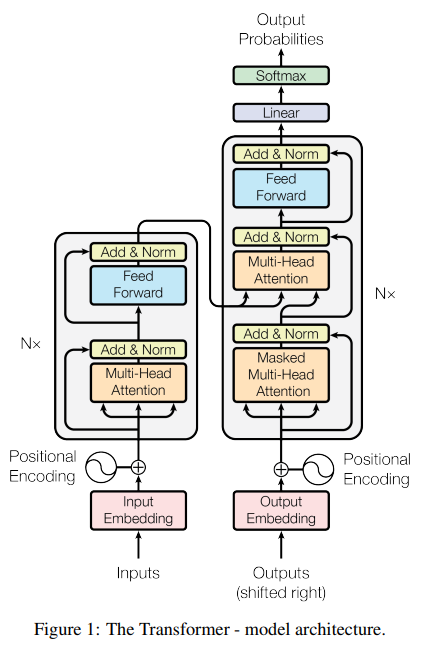
\includegraphics[width=0.5\linewidth]{figures/vasvani_transformer.png}

    % Improve caption formatting for papers
    \caption{A figure from \cite{vaswani2023attentionneed} showing the traditional encoder-decoder transformer architecture \textcolor{red}{[place holder - will add new architecture figure]}}
    \label{fig:vasvani_trans}
\end{figure}

\subsection{Conditional latent diffusion model}

Latent representations produced by the transformer-based auto-encoder are flattened and paired with their corresponding condition parameters to train a conditional diffusion model. We adopt the diffusion framework provided by the smalldiffusion package \cite{Yuan2025_smalldiffusion}, using its standard noise scheduling, training objectives, and sampling procedures. Modifications are introduced only in the conditioning mechanism and denoising network to enable modeling of multiple continuous design conditions.

In contrast to the standard neural network based denoising model implemented in the smalldiffusion package, we employ feature-wise linear modulation (FiLM) \cite{perez2017filmvisualreasoninggeneral}, to accommodate continuous design conditions. These condition values are first embedded using a small neural network and then passed on to FiLM layers for modulating the intermediate layer outputs.

This conditional diffusion model is then trained using the standard classifier-free guidance formulation implemented in the smalldiffusion package. Training minimizes a mean squared error loss between the predicted and true noise over a predefined noise schedule, with the conditioning inputs randomly dropped and replaced by a null condition. During inference, guided sampling is performed by combining conditional and unconditional predictions using a guidance scale, allowing explicit control over influence of conditioning. Generated latent samples are then reshaped to reverse flattening and are subsequently decoded using the decoder previously described, and put through the post-processing pipeline outlined in figure \ref{fig:model_training_pipeline}


